\documentclass{article}
\usepackage[utf8]{inputenc}
\usepackage{hyperref}
\usepackage[T1]{fontenc}
\usepackage{lmodern}
\usepackage{cmap}
\usepackage[utf8]{inputenc}
\usepackage[english]{babel}
\usepackage{graphicx}
\usepackage{caption}
\usepackage{subcaption}

\title{Bay Area Bike Share Data Analysis}
\author{Maxim Kovalev\\\href{mailto:maxim.kovalev@2007.auditory.ru?subject=Bay Area BikeShare Data Analysis}{maxim.kovalev@2007.auditory.ru}}
\date{May 2015}


\newcommand{\fix}{\marginpar{FIX}}
\newcommand{\new}{\marginpar{NEW}}


\begin{document}

\maketitle

\begin{abstract}
In this report I outline the findings of analyzing Bay Area BikeShare data, and come to the conclusion that not only more bikes are needed for the system to function, but also more docks than bikes are needed. For key findings, refer to sections \ref{sec:available} and \ref{sec:conclusions}, although additional findings are presented elsewhere.
\end{abstract}

\section{Tech specs}
Data for this report was obtained from Bay Area BikeShare Open Data Challenge (although this is not a competition submission), and as of May 11, 2015 could be obtained here: \url{http://www.bayareabikeshare.com/datachallenge-2014}.

Code for all the analytics is published under GPLv3, and can be found here: \url{https://github.com/maxikov/bikedatan}. This repository contains the entire distribution needed to run the code, except for the data itself. To run the code, extract data from ``August 2013 - February 2014'' archive from BikeShare to ``data/02/'' subfolder, and ``March 2014 - August 2014'' to ``data/08''.

This code runs on Python 2.x interpreters, 2.7 or older, but not 3.x. In addition to the standard library, it uses numpy, matplotlib, and mpl\_toolkits.basemap.

\subsection{Zip code data set}

In order to work with the data about users' home zip codes, I downloaded an extra data set of coordinates of US zip codes from \url{https://www.gaslampmedia.com/download-zip-code-latitude-longitude-city-state-county-csv/}. This data set isn't fully complete, which I partially fixed by manually adding some of the commonly occurring in the main data set zip codes, but for future work a more complete set may be benefitial.

\section{Scope}

In this report I primarily focus on the data that can be derived by incorporating the information about users' home coordinates, approximately derived from the zip code. As far as I can tell, none of the Open Data Challenge winners has done that. On contrary, \cite{mousebird} and \cite{planetbabs} have created beautiful and informative tools for studying the graph of rides, so I decided against replicating those already achieved results.

\section{Data set overview}
\label{sec:dsover}

Bay Area BikeShare (BABS) provides 4 data sets collected over 6 months of their operation (with an addition of the identically structured data sets for 6 more months):
\begin{enumerate}
	\item
		Trip data -- for every ride done on BABS bikes, they provide the time this ride was made, ID of the departure station, and ID of the arrival station. In addition, for those rides made by annual subscribers, subscriber's home zip code is provided.
	\item
		Station data -- for every station, referred to by its ID, latitude and longitude is provided, along with the time the station was put into operation.
	\item
		Weather data -- for every day, various meteorological parameters are provided.
	\item
		Rebalancing data -- for every station, once a minute an observation is made how many bikes it has, and how many available docks it has.
\end{enumerate}

\begin{figure}
	\centering
	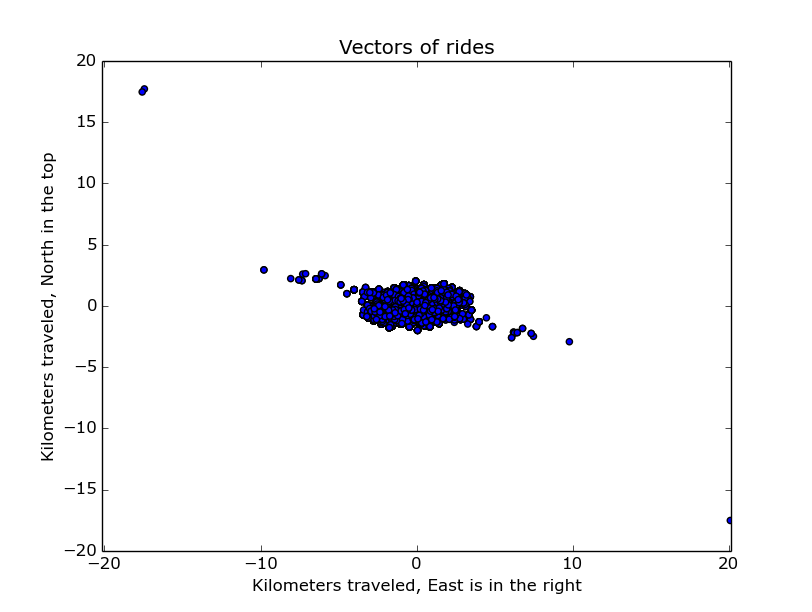
\includegraphics[width=0.9\textwidth]{../travel_vector.png}
	\caption{Distribution of travel vectors, in kilometers}
	\label{fig:travelvector}
\end{figure}

\begin{figure}
	\centering
	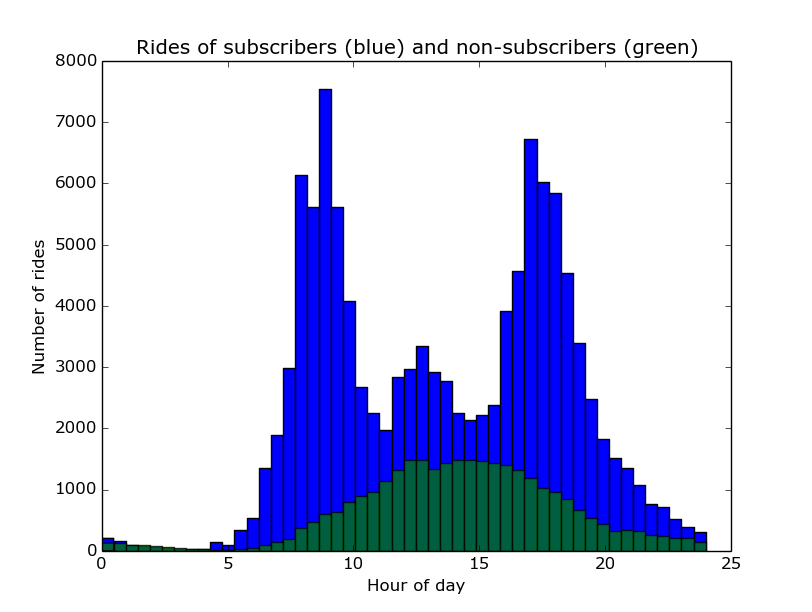
\includegraphics[width=0.9\textwidth]{../time_of_day_sub_not_sub.png}
	\caption{Rides by subscribers and non-subscribers every day}
	\label{fig:sns}
\end{figure}

\section{Trip vectors and times}
Figure \ref{fig:travelvector} reveals that relative to the station of departure, riders have a strong tendency to travel from East to West and back more than from North to South. Geographically, this pattern would be expected from San Fransisco, and \cite{babs} confirms that SF accounts for 90\% of all the rides, thus dominating the data set.

As \cite{babs} has also shown, and I confirmed in Figure \ref{fig:sns}, annual subscribers dominate the data set, and exhibit a vastly different pattern compared to non-subscribers. Namely, the pattern of subscriber activity matches the scheme ``morning commute -> going out for lunch -> evening commute'', whereas non-subscribers ride far less, and smoothly peak in the mid-day, matching the pattern of tourist or leisure activity.

\begin{figure}
        \centering
        \begin{subfigure}[b]{0.5\textwidth}
                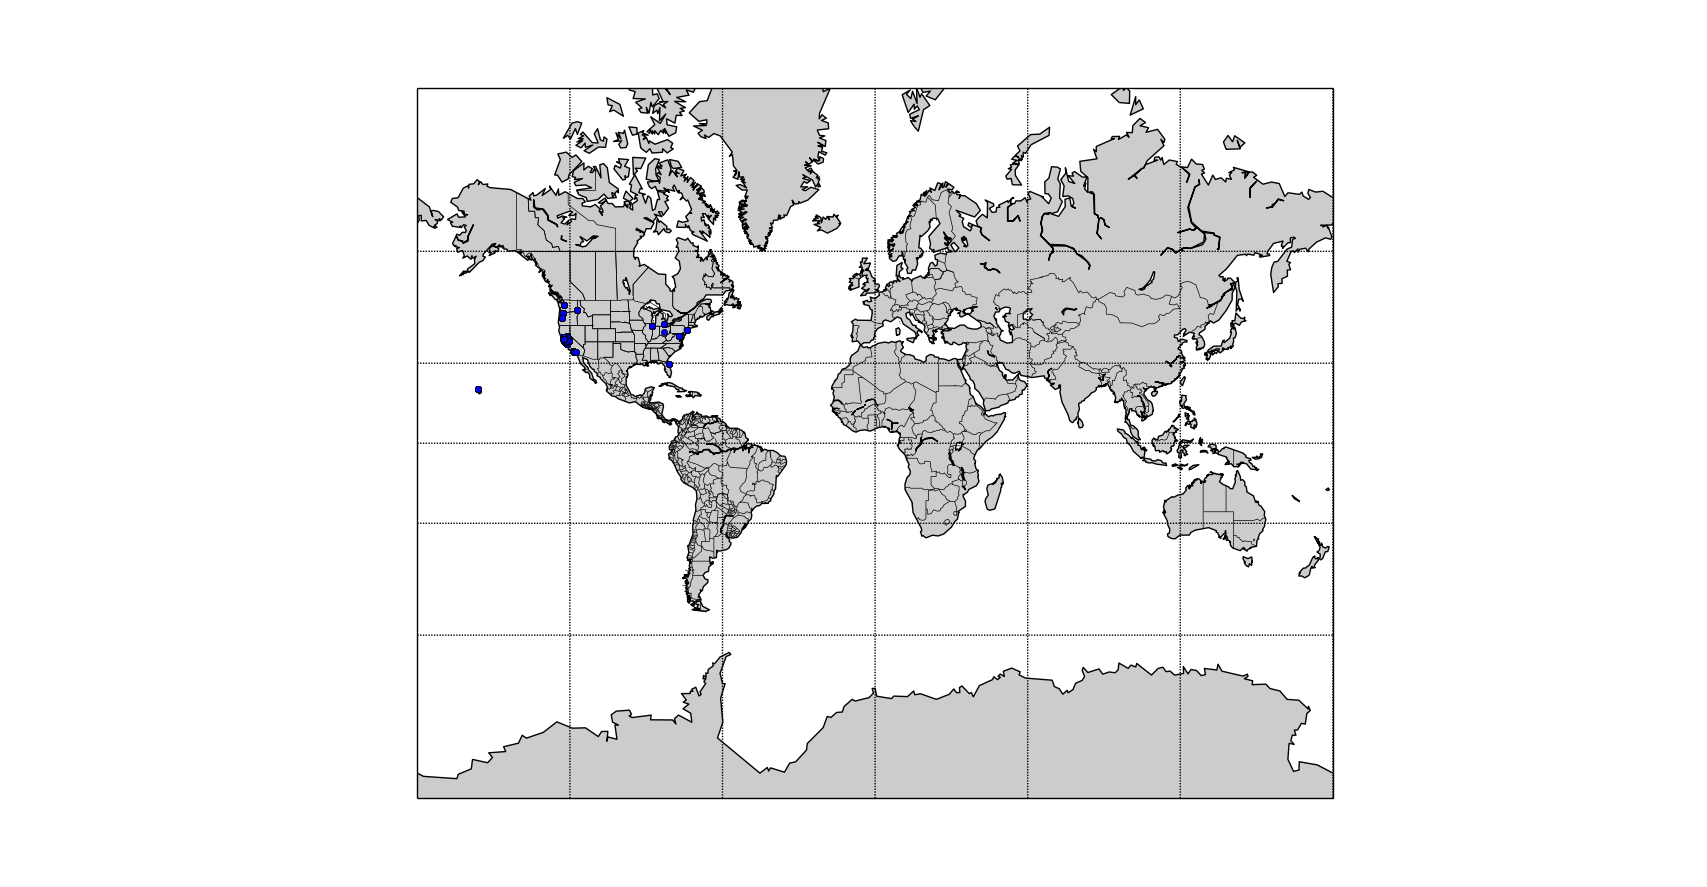
\includegraphics[width=\textwidth]{../home_zips_world.png}
                \caption{On the world map}
                \label{fig:homezips:world}
        \end{subfigure}%
        ~ %add desired spacing between images, e. g. ~, \quad, \qquad, \hfill etc.
          %(or a blank line to force the subfigure onto a new line)
        \begin{subfigure}[b]{0.5\textwidth}
                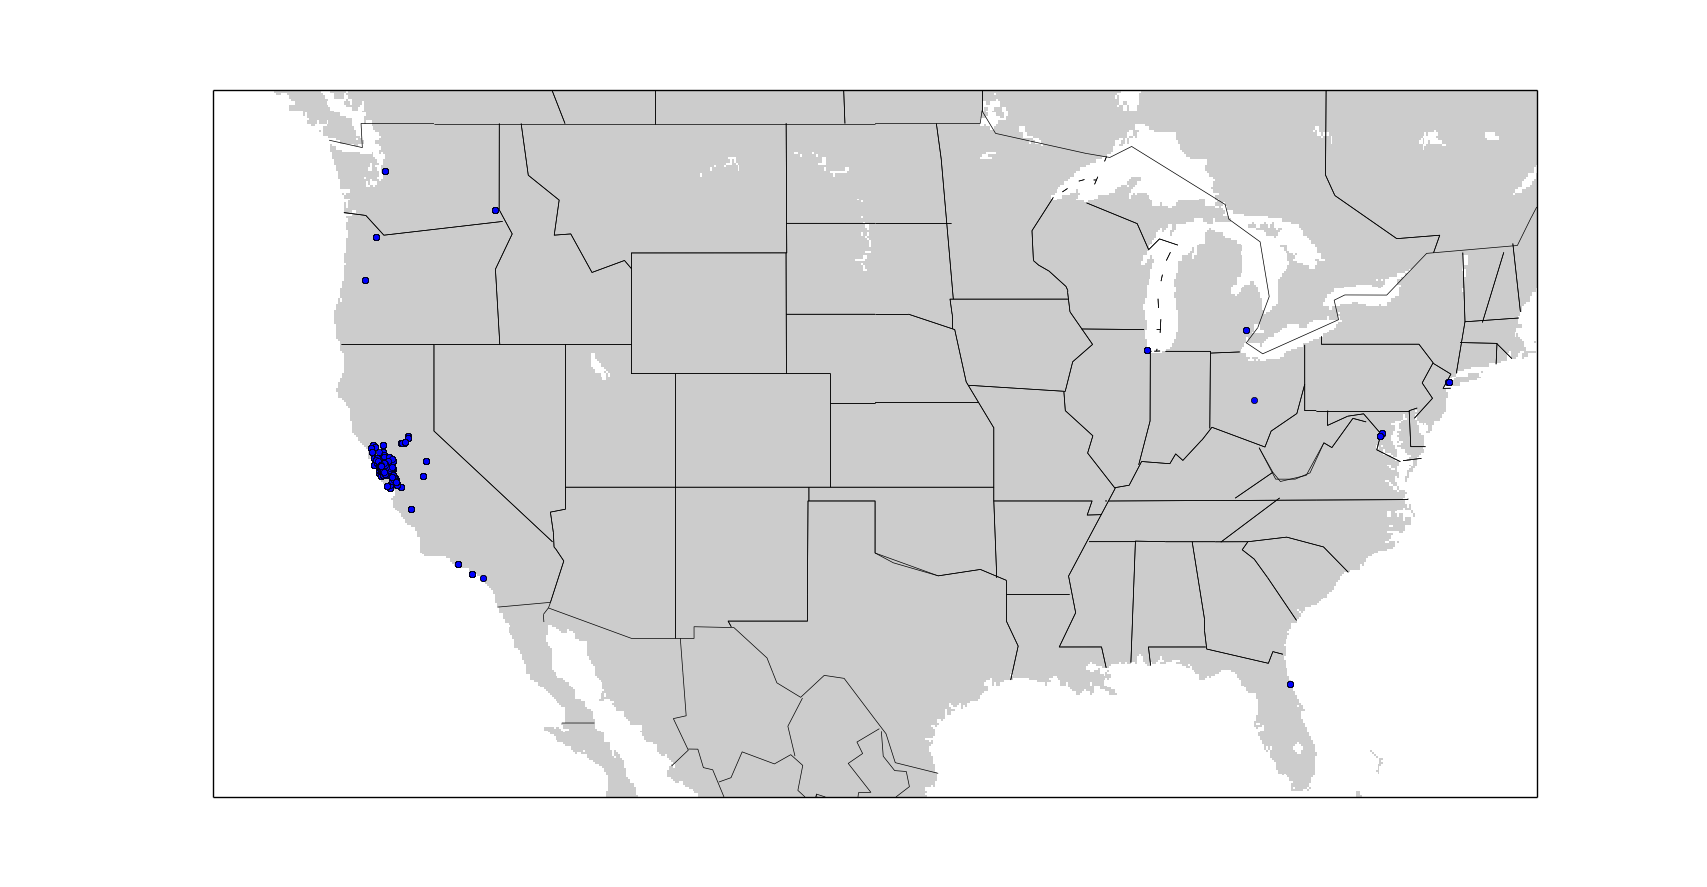
\includegraphics[width=\textwidth]{../home_zips_usa.png}
                \caption{On contiguous states map}
                \label{fig:homezips:usa}
        \end{subfigure}
        ~ %add desired spacing between images, e. g. ~, \quad, \qquad, \hfill etc.
          %(or a blank line to force the subfigure onto a new line)
        \begin{subfigure}[b]{0.4\textwidth}
                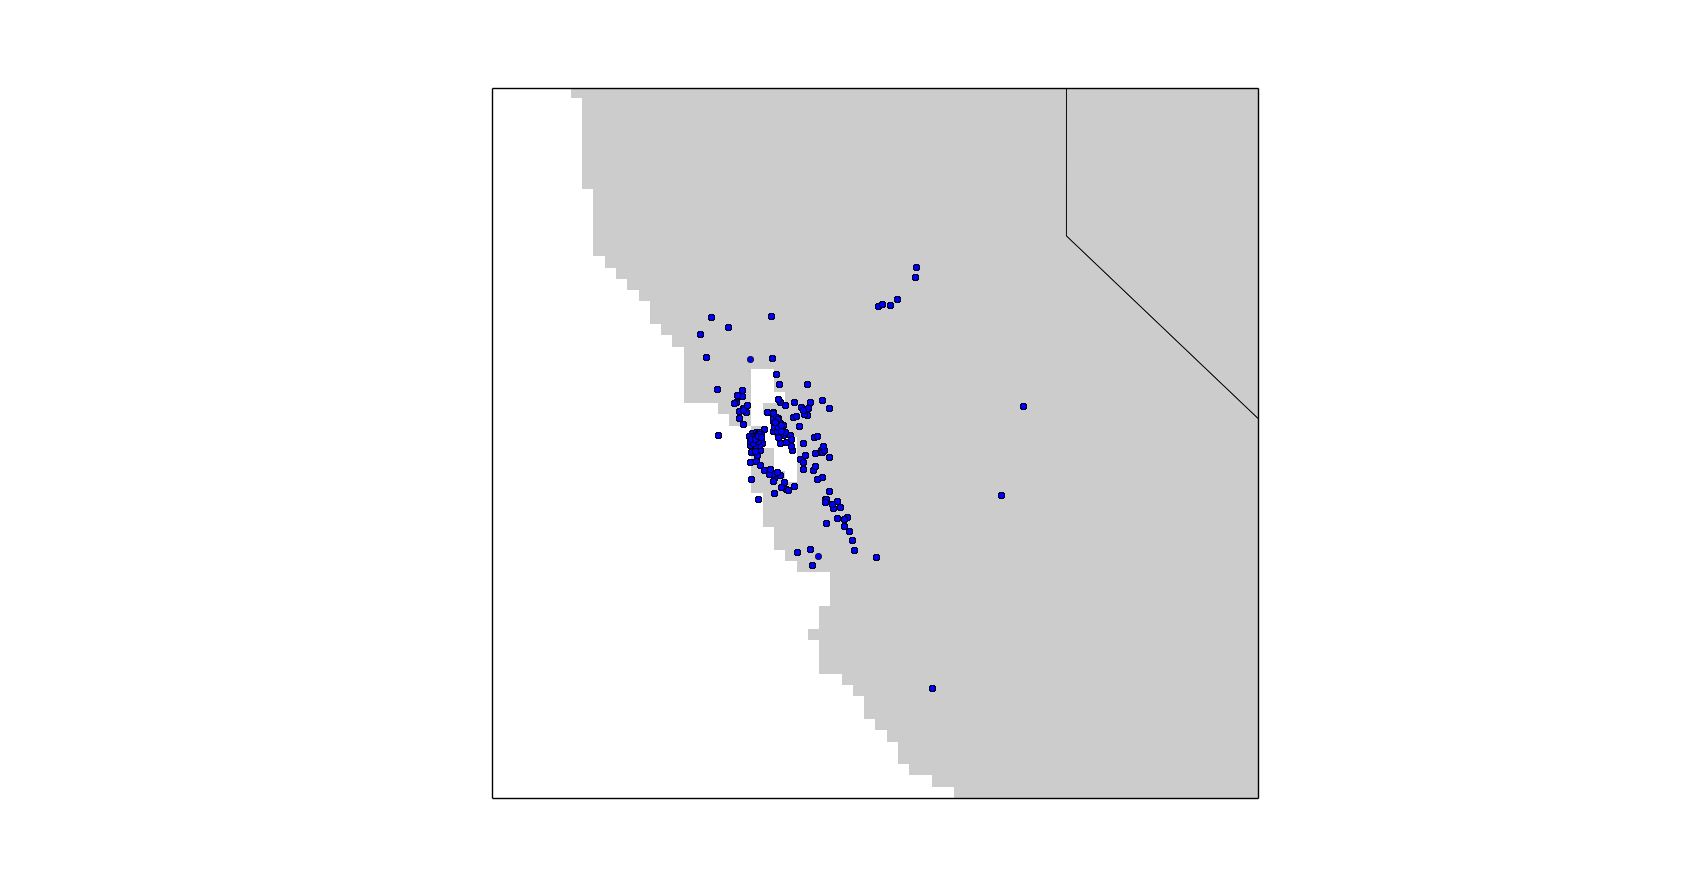
\includegraphics[width=\textwidth]{../home_zips_norcal.png}
                \caption{On Northern California map}
                \label{fig:homezips:norcal}
        \end{subfigure}
        \begin{subfigure}[b]{0.4\textwidth}
                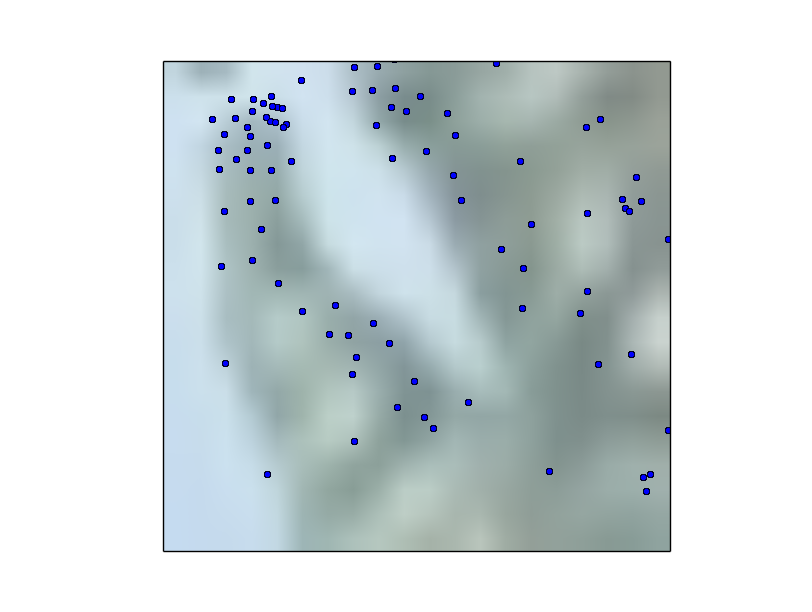
\includegraphics[width=\textwidth]{../home_zips_bay_area.png}
                \caption{On Bay Area map}
                \label{fig:homezips:}
        \end{subfigure}
        \caption{Coordinates of home zip codes of subscribers}
        \label{fig:homezips}
\end{figure}

\section{Home address distribution}

For annual subscribers, home zip codes are provided. According to \cite{babs}, 80\% of rides are done by the subscribers, which warrants studying them as highly representative of the entire user base. Figure \ref{fig:homezips} shows where the subscribers live -- unsurprisingly, they mostly live in the Bay Area, and are particularly concentrated in the Peninsula, although statistically significant portion of them also lives elsewhere in the Northern California, and some outliers can be found in the entire country.

\begin{figure}
	\centering
	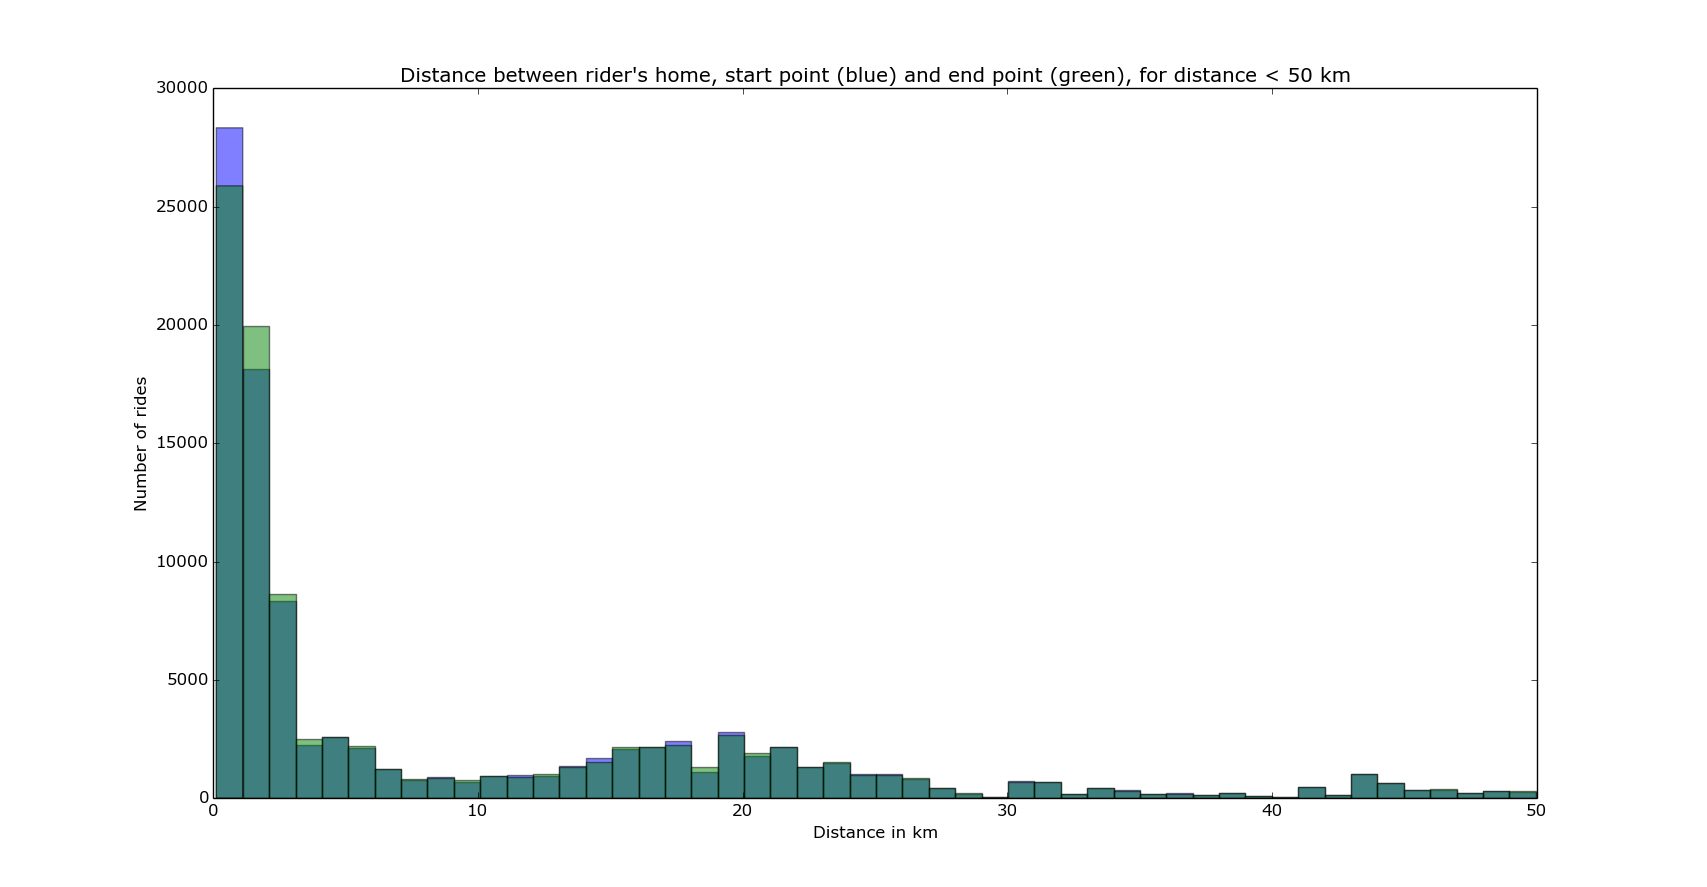
\includegraphics[width=\textwidth]{../start_end_home.png}
	\caption{Distribution of distances from user's home to the start point of the trip (blue) and the end point (green)}
	\label{fig:startendhome}
\end{figure}

\section{Distance between home and bike stations}

Figure \ref{fig:startendhome} show the distribution of distances from user's home to the start point of a ride and the end point. By incorporating a 50 km threshold, I make sure to only count Bay Area residents. The distribution is noticeably multimodal, with the largest peak near zero, and the smaller but still significant peak around 20 kilometers. Incidentally, this is the distance between centers of San Francisco and Oakland, which could be a coincidence, but given the 90\% dominance of within-SF rides, it could well indicate that a significant number of people commute from East Bay by BART, and then take a bike.

The distributions of distances from home to end and to start of the travel follow each other very closely. This is not surprising, given that, according to Figure \ref{fig:travelvector}, travels tend to be short, and both points are likely to be close to home. Furthermore, the accuracy of positioning by zip code may be not high enough to really distinguish such small differences -- it may well be the case that both the start and the end points are within the same zip code. However, Figure \ref{fig:ridestofromhome} clearly demonstrates that far more rides are identified as ``from home'' in the morning, and ``to home'' in the evening, supporting the claim that such classifier adequately discovers the ride direction.

However, a small difference may be noticed near the left border of the distribution. Namely, more rides apparently end start right next to the home than they end, and more rides end slightly faraway from home than they begin. Specifically, there are 57515 rides that start near home, and 55890 ones that end near home. In the real world, this can translate into the hypothesis that people prefer to bike in the morning, but some other form of transit in the evening. This is supported by Figure \ref{fig:sns}, in which more travels can be seen in the morning than in the evening.

\begin{figure}
	\centering
	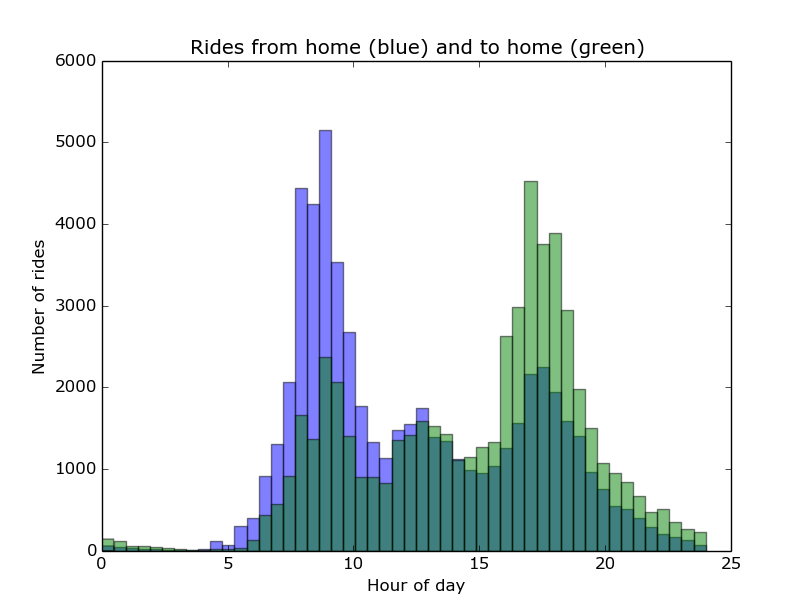
\includegraphics[width=0.8\textwidth]{../rides_from_home_to_home.png}
	\caption{Number of rides per time of the day. Blue are the rides where the user's home is closer to the start point of the ride, and green are the opposite}
	\label{fig:ridestofromhome}
\end{figure}

\begin{figure}
	\centering
	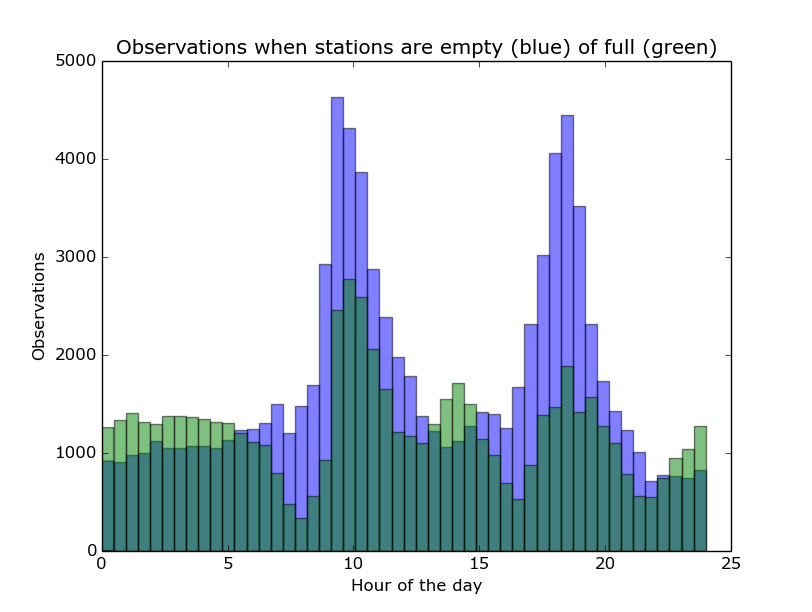
\includegraphics[width=0.8\textwidth]{../empty_full_stations.png}
	\caption{Observations of empty and full stations. Observations are made every minute, so for each bar the height is proportional to the sum of the portions of time each station has stayed empty or full. }
	\label{fig:emptyfull}
\end{figure}

\section{Ride directions and station availability}
\label{sec:available}

Figure \ref{fig:emptyfull} represents the station availability throughout the day. As mentioned in section \ref{sec:dsover}, every minute the system reports for each station the number of bikes and docks available. Simply counting such reports where stations are empty or full makes a good proxy for how bad the situation with the lack of bikes is. Namely, for a particular station, in a particular period of time, this will yield a number of minutes when the station was empty (or full). If this number is high, then the station is empty most of the time, and this is probably a problem to be addressed. On the other hand, if the number is low, the users can easily wait. Adding these numbers for all stations gives us the overall picture of how bad the situation with the lack of bikes is.

Since every bike must be put to a dock after the ride, the situation of the station being full is just as bad as the lack of bikes: it forces the rider to walk to or from another station. Therefore, high percentage of both empty and full stations should be addressed.

The most interesting conclusions can be drawn from comparing Figure \ref{sec:dsover} to Figure \ref{fig:ridestofromhome}.

\begin{itemize}
	\item
		The peaks of full stations are right after the peaks of commutes. This could imply two-way causation here: large demand for bikes obviously causes a large portion of empty stations, but then the lack of bikes (rather than the decrease in demand for them) could be causing the decline in the number or rides. If this is the case, it means that the demand for bikes exceeds the supply, and surge pricing or increasing the number of bikes would lead to marginal revenue increase.
	\item
		The morning peak of full station is clearly higher than that in the evening. This matches the pattern of riders coming from sparsely populated parts of San Fransisco to its commercial areas, which take less space. Thus, the concentration of bikes increases, and that causes dock congestion in these areas. In the evening, on the other hand, the demand for bikes is just as high as in the morning, but they get dissipated to a greater area, thus overloading less docks.
	\item
		Commuter peaks of empty stations coincide with the peaks of full stations. During the lunch time, however, there's a local minimum of empty stations, and a local maximum of full stations. This could mean that the areas where people go for lunch are even more concentrated than their work. Thus, without creating a lot of empty stations, people manage to overload those few stations that are close to the restaurants. This could simply be fixed by adding more docks (but not necessarily bikes) to such ares.
	\item
		Slightly before the peaks of empty stations, there are local minima of full stations. This could mean that some stations are unnecessarily full by default, and taking bikes from them actually relieves the congestion, before it's caused by concentrated traffic elsewhere.
\end{itemize}

\section{Conclusions}
\label{sec:conclusions}
Although highly speculatively, it can be concluded that commuter traffic suffers from both the lack of available bikes, and the lack of available docks. The lack of dock appears to be an even more serious problem during the lunch time, presumably at the stations near restaurants. This could also signify that the area where people live is larger than that where they work, and the area where they go to lunch is even smaller. Given that commuter traffic temporarily relieves the dock congestion, it can be speculated that the system will benefit from having more docks than bikes at most (if not all) stations. On the other hand, some stations (presumably near large transportation centers like Caltrain $4^{th}$\&King and BART Embarcadero) would benefit from having significantly more bikes, and this is likely to cause marginal revenue increase. On the other hand, the data suggests that morning commuter traffic tends to concentrate more than evening traffic, which, along with the usual proximity of stations to the users' homes, could indicate that connections from trains could be not as important as the wide network coverage

\section{Future work}
The findings of this study indicate several ways to improve it further. As mentioned before, a more complete database of zip codes could make the findings more reliable. In addition, it would be worthwhile to investigate the difference between weekend and weekday traffic -- particularly, to confirm which one generates more revenue. Most conclusions about the congestion are drawn from common sense considerations, and would benefit from a more data-driven approach. Particularly, building a heat map of congestion, and studying the graph of rides to figure which stations could benefit form more docks and more bikes, and in which proportion, could yield actual business proposals.

\bibliographystyle{apa}

\begin{thebibliography}{9}

\bibitem{mousebird}
\url{http://mousebirdconsulting.blogspot.ru/2014/04/bay-area-bike-share-data-challenge.html}

\bibitem{planetbabs}
\url{http://www.bayareabikeshare.com/assets/pdf/Bjorn.pdf}

\bibitem{babs}
\url{http://thfield.github.io/babs/}


\end{thebibliography}




\end{document}

